\section{Motivação}
\label{sec:Motivação}

A proposta deste trabalho é criar um ambiente consciente, onde o contexto
locativo oriundo do posicionamento remoto de cada dispositivo móvel é
administrado e divulgado pelo prédio conectado ao invés da auto-localização do
aparelho, pois:

\begin{alineas}

	\item Uma vez encontrada a localização, é mais fácil propagar esta informação do
ambiente para o aparelho em comparação ao autoposicionamento, pois a negociação
entre o ambiente e o aparelho é nula quando o primeiro contém a informação- o
ambiente sempre disponibilizará uma informação coletada para o gerador desta
informação;

	\item Pode-se lidar com grande heterogeneidade de dispositivos, uma vez
que cada um deles não precisa se adaptar para cada mudança de ambiente;

	\item Este tipo de informação já é contida nos históricos de cada Ponto de
	Acesso \emph{Wi-Fi} (AP - \emph{Access Point}), porém:

	\begin{alineas}

		\item Geralmente sem uso - poucas são as aplicações que usam a
		localização obtida pelo AP;

		\item Com granularidade insuficiente para uso em aplicações
		contextualizadas;

		\item geralmente não disponibilizada pelos APs.

	\end{alineas}

	\item Uma vez instalado um PS deste gênero, a quantia de dispositivos que
	ele pode localizar fica limitada apenas pela rede física anteriormente
	instalada;

	\item Economia de hardware quando menos é exigido de cada dispositivo móvel.

\end{alineas}

Nota-se também que mesmo com a quantidade prevista de 5 dispositivos IoT por
pessoa em média, estes seriam beneficiados sempre que utilizados no ambiente
conectado proposto.

\begin{figure}[htb]
	\caption{\label{fig-projeto}Modelo das camadas }
	\begin{center}
		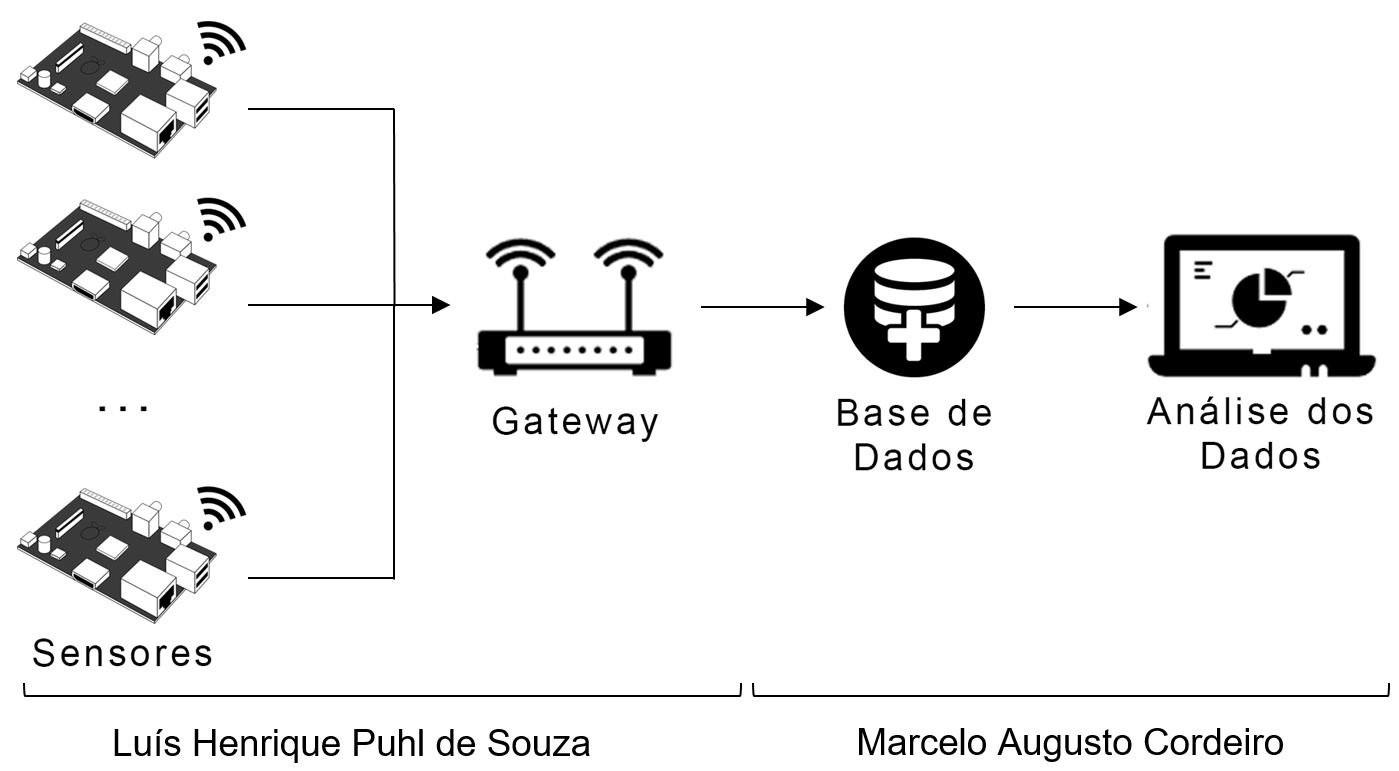
\includegraphics[width=1\textwidth]{012-justificativa/img/projeto.jpg}
	\end{center}
	\legend{Fonte: Marcelo Augusto Cordeiro \cite{Cordeiro2016}}
\end{figure}

A Figura \ref{fig-projeto} apresenta a arquitetura simplificada de uma aplicação
IoT, e no detalhe inferior a relação deste projeto com o do aluno Marcelo Augusto
Cordeiro, também do Bacharelado de Ciências da Computação, que é também membro do
ambiente de testes LTIA (Laboratório de Tecnologia da Informação Aplicada) da Unesp de Bauru
e do mesmo edital para obter o título de bacharel.
